%% LaTeX2e class for student theses
%% sections/evaluation.tex
%% 
%% Karlsruhe Institute of Technology
%% Institute for Program Structures and Data Organization
%% Chair for Software Design and Quality (SDQ)
%%
%% Dr.-Ing. Erik Burger
%% burger@kit.edu
%%
%% Version 1.3.2, 2017-08-

\chapter{Evaluation}
\label{ch:eval}
After we evaluated the created case study in \autoref{ch:cocome} and \autoref{ch:apllMethod}, in this chapter the procedure (\autoref{ch:method}) and the used modeling language (PCM \cite{PCM}) are evaluated. The evaluation are also based on a GQM-plan \autoref{GQM_Expl}. The plan for the whole evaluation can be seen in \autoref{GQMPlan}. \\ First, we conduct the evaluation for the applicability of the presente dprocedure, then the expressibility of the modleing language. Afterwards, we summarize the results for the created case study. To conclude the chapter, we discuss the \textit{threats to validity} (\cite{TtoV}).

\begin{figure}
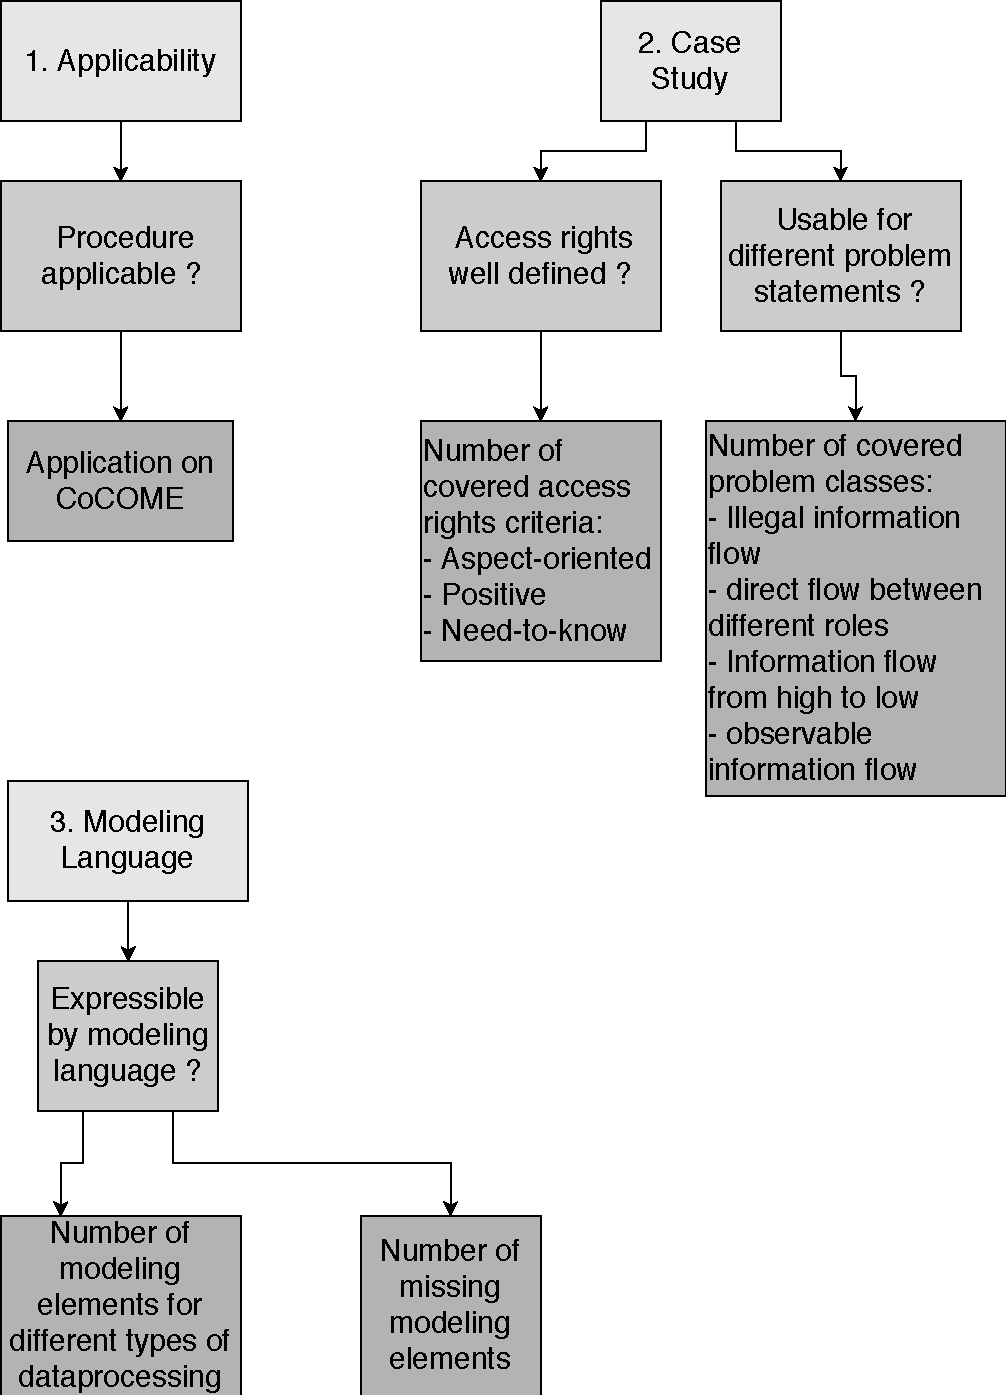
\includegraphics[scale=.8, origin=c ]{logos/OverviewEval.pdf}
\caption{The GQM plan for the three parts of the evaluation. Each part is divided into }01
\label{GQMPlan}
\end{figure}

\section{Goal: Applicability of the introduced procedure}
The first aspect we are evaluating is the applicability of the introduced procedure to create case studies from software systems. We evaluate the applicability to verify if its possible to create case studies that later may be used to evaluate approaches for a data-based privacy analysis. The examination if the quality of the created study is sufficient is a separate part and has to be done on a case-by-case basis.  
\subsection{Question: Is the introduced method applicable to an actual system?}
To verify if the goal is achieved, we check if the introduced procedure is applicable to a software system that abstracts the selling process and warehousing of a supermarket group. The metric to answer the question is a successful application to an actual system.  
\subsubsection{Application to the CoCoME system}
The system we chose to apply the method on is CoCoME. We applied the procedure not the whole CoCoME system but only to an excerpt of it. The application to the excerpt and resulting case studies is conducted in \autoref{ch:cocome} and \autoref{casestudysystem}.\\ We successfully applied the procedure to an actual system and created a case study. Therefore, we conclude that the procedure is applicable.
%\section{Usability of the created case study for data-based privacy analysis}
%\label{usage_DBPA}
%The next aspect we evaluated the usability of the created case study. A case study is not useful if it does not meet criteria. The criteria ensure that the case study is in a state where it can be used for data-based data privacy analysis. To ensure this, we evaluate two different parts of the case study. First, we evaluate the defined access rights, then the defined data flows. 


\section{Goal: Expressiveness of data-centric PCM}
In this part, we evaluate the modeling language that is used for the case study. To model the case study, technically speaking, it have to be possible to add two extensions to the system model. First the data flows and ,Secondly ,the defined ACM.\\ We chose to use data-centric PCM as the modeling language % ref auf foundations
By default it is not possible with data-centric PCM to extend models by data flows and an ACM. Therefore we went for the meta-model extension for data-centric PCM from Seifermann \cite{MMextension}. So, this part of the evaluation will mainly focus on the meta model extension for data-centric PCM. 

\subsection{Is the created case study expressible with data-centric PCM ?}
To verify, if the case study is expressible with data-centric PCM, we ar eusijgn two metrics. First we measure which elements are available and then which elements are missing.
\subsubsection{Number of available elements to model the different types of data processing}
The main focus is to verify, if the created case study is expressible with data-centric PCM. We check if it is possible to model all defined operations in the OpM. %ref OpM !!! 
This is also done in a checklist manner.
We defined four operations for the case study in the OpM: transmission of data, alternation of data, operations for relational algebra and operations to model user interaction. 

\paragraph{Transmission data}
This operation describes if components transmit data. An operation for this available in the meta model extension.

\paragraph{Alternation of data}
This is a larger type of operations. All in all, this type describes the alternation of data. This includes
creation of data, merging many points in, for example, into list or set, the splitting of data, like lists, in the single data, etc. With the alternation of data it can happen that the class of data is changed and thus the applying access rights change. To describe the change of the applying access rights an operation is available in the meta model extension. 

\paragraph{Operations relational algebra}
This type of data processing describes the manipulation of database or data requested from databases. The operations for this are available in the meta model extension. 

\paragraph{I/O- operations}
To model the user interactions an operation is also available.


\subsubsection{Number of missing elements for the different }
Currently it is not possible to store the ACM in the same system model. It is possible to define access rights for each data in each component for each role. First, for each data a new access right has to be defined and , secondly, it is not or only with disproportionate effort possible to swap out the access rights or generating the ACM form the model. For the fact, we created our case study \textit{aspect-oriented} (see \cite{}) the current modeling contradicts the concept. Therefore, a model element for the ACM is missing.
\subsubsection{Summary: expressiveness of data-centric PCM}
The summary of the both metrics is shown in 
\begin{table}
\begin{tabular}{|c|c|}
\hline 
Meta model  & possible ? \\ 
\hline 
relational algebra & \cmark \\ 
\hline 
I/O operations & \cmark \\ 
\hline 
Transmission of data & \cmark \\ 
\hline 
Change of access rights & \cmark \\ 
\hline 
Alternation of data & \cmark \\ 
\hline 
ACM in system model & \xmark \\
\hline
\end{tabular} 
\caption{Summary for the evaluation for the modeling language.}
\label{PCM_eval_sum}
\end{table}
\section{Evaluation of the created case study}
%schon passiert, hier nur eine kurze zusammenfassung
\subsection{Summary}

%tabellen hie reinfügen 
\section{Discussion}
%After all the evaluations are conducted, we discuss the findings. This discussion will be divided into three parts. Each parts covers one of the evaluation aspects shown in \autoref{GQMPlan}.\\
%We were able to verify that the method is applicable to a system that models a pickup shop. The method should also be applied to other systems. Possible other systems are flight booking systems, food suppliers, etc. The weakness in this part of the evaluation is that the method has not been applied often enough to different systems to make a statement about its applicability.\\
%In the next part, the evaluation results of the access rights and data flows are discussed. First, the defined access rights in the case study. We evaluated based on predefined criteria by Evered and Bögeholz \cite{CaseStudyAndAccessrigths} the access rights. Not all criteria were applicable to the case study, because for some criteria one need running code which is not in the scope of the case study. Other criteria weren't applicable due to time constraints. All in all, as shown in \autoref{eval_AR}, we achieved with our definition of the access rights all three criteria. There is surely some work to be done to allow to check more criteria, like conducting a survey for the criteria clear and concise. For the criteria fundamental and efficient a deployment of CoCoME which includes the access rights is needed. The evaluation of the access rights has to be taken with a grain of salt. Since the access rights depend on the security-relevant data and the roles defined in the system, they must be reevaluated if something has changed.  The evaluation is therefore only a snapshot of the current quality of the access rights. Next, we discuss the evaluation for the different covered information flow classes. We achieved to cover two of the four information flow classes, which is a pretty solid. As we see it, the desirable state is to cover all information flow classes in width and depth. Width means that at least each class is covered by at least one data flow. Depth means that for each class a data flow is defined that is illegal for the class and one that it is not.As shown in \autoref{eval_DF}, we only cover two information flow classes. 
%At last we discuss the results for our modeling language PCM. We defined five types of data processing and evaluated whether they are possible to model in PCM. The result is shown in \autoref{eval_MM}. As shown, all types of data processing are modeled. Therefore, we conclude it is be possible to model all created case studies with PCM. But it is not possible to store the ACM in the same model. 



%\begin{table}
%\begin{tabular}{|c|c|}
%\hline 
%Access Rights & fulfilled ? \\ 
%\hline 
%Aspect-oriented & \cmark \\ 
%\hline 
%Positive & yes \\ 
%\hline 
%Need-to-know & yes \\ 
%\hline 
%\end{tabular} 
%\caption{Overview of the evaluation result for the access rights.}
%\label{eval_AR}
%\end{table}

%\begin{table}
%\begin{tabular}{|c|c|}
%\hline 
%Data flow & fulfilled \\ 
%\hline 
%Illegal information flow & yes \\ 
%\hline 
%Information flow from high to low & yes \\ 
%\hline 
%Observable information  flow & no \\ 
%\hline 
%Direct information flow between roles & no \\ 
%\hline 
%\end{tabular} 
%\caption{Overview over the evaluation result for the data flows.}
%\label{eval_DF}
%\end{table}
 
\begin{table}
\begin{tabular}{|c|c|}
\hline 
Meta model  & possible ? \\ 
\hline 
relational algebra & \cmark \\ 
\hline 
I/O operations & \cmark \\ 
\hline 
Transmission of data & \cmark \\ 
\hline 
Change of access rights & \cmark \\ 
\hline 
Alternation of data & \cmark \\ 
\hline 
ACM in system model & \xmark \\
\hline
\end{tabular} 
\caption{Overview over the results for the evaluation of PCM.}
\label{eval_MM}
\end{table}
To conclude the evaluation, one can say that we introduced an applicable method for a certain typ eof systems to create data flows for a data-based privacy analysis. For the sample case study, we say it is a proof-of-concept, because only two class of information are modeled. The defined access rights are well defined in the current evaluation, but it is imperative to apply the other criteria to get a more complete picture. It must also be said that access rights are relatively volatile, as there is a need to check even small changes in the system. At last, the used modeling language is able to model all types of data processing and is therefore usable for data-based privacy analysis. The only throwback for the modeling language is that the ACM must be stored separately, this may lead to inconsistency and should be fixed soon.

\section{Threats to validity}
In this section we discuss possible threats to the validity of the evaluation. %hie rmal von HEinrich klauen, eventuell
 The threats are divided into four categories: internal validity, external validity, construct validity and conclusion validity.

